\documentclass{article}

\usepackage{amsmath}
\usepackage{graphicx}
\usepackage{hyperref}
\usepackage[utf8]{inputenc}
\usepackage{lipsum}
\usepackage{multicol}
\usepackage{titling}
\usepackage[a4paper]{geometry}
\usepackage{tikz}
\geometry{
    left=20mm,
    top=20mm,
}
\renewcommand{\thesection}{\Roman{section}}
\renewcommand{\thesubsection}{\Roman{subsection}}
\title{\LARGE \textbf {\huge{Tugas Probabilitas dan Statistika}}}
\author{
    M Rizqi R\\
    20051204034\\
    Teknik Informatika 2020 B\\
    Universitas Negeri Surabaya\\
}
\date{\today}

\begin{document}
    \maketitle
    \section{Variabel}
    S = Himpunan Semesta\\
    P = Perokok\\
    K = Alkohol\\
    G = Gaya hidup tidak sehat\\
    \section{Data}
    \begin{enumerate}
        \item \( n(S) = 40.000\)
        \item \( n(P) = 29.000\)
        \item \( n(K) = 25.000\)
        \item \( n(G) = 30.000\)
        \item \( n(P \cap K) = 22.000\)
        \item \( n(P \cap G) = 24.000\)
        \item \( n(K \cap K) = 20.000\)
        \item \( n(P \cap K \cap G) = 20.000\)
    \end{enumerate}
    \section{Ditanya}
    Perokok tapi tidak kecanduan alkohol = \( n(K^c \cap (A-B)^c)\)\\
    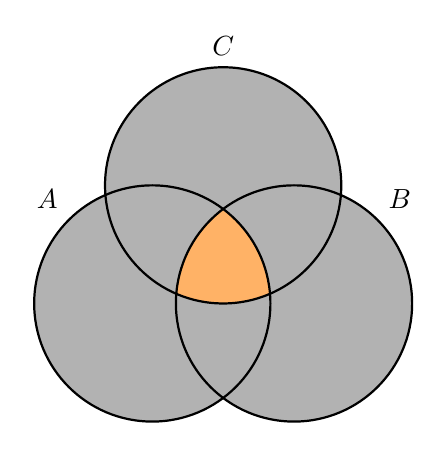
\begin{tikzpicture}
        [thick,
    set/.style = {circle,
        minimum size = 3cm,
        fill=black!30}]
 
% Set A
\node[set,label={135:$A$}] (A) at (0,0) {};
 
% Set B
\node[set,label={45:$B$}] (B) at (1.8,0) {};
 
% Set C
\node[set,label=$C$] (C) at (0.9,1.5) {};
 
% Intersection
\begin{scope}
    \clip (0,0) circle(1.5cm);
    \clip (1.8,0) circle(1.5cm);
    \clip (0.9,1.5) circle(1.5cm);
    \fill[orange!60](0,0) circle(1.5cm);
\end{scope}
 
% Circles outline
\draw (0,0) circle(1.5cm);
\draw (1.8,0) circle(1.5cm);
\draw (0.9,1.5) circle(1.5cm);
    \end{tikzpicture}
    \section{Jawaban} 
\end{document}













